\documentclass[a4paper,10pt]{article}
\usepackage[dvips]{color,graphicx}
\usepackage[dvips, bookmarks, colorlinks=false]{hyperref}

%opening
\title{Math650 Homework 4}
\author{Yu Huang}

\begin{document}

\maketitle

\begin{abstract}
t test, randomization, distribution of t-statistic
\end{abstract}

\section{Introduction}
Study the role of randomization in the distribution of the t-statistic and calculation of p-value.

\section{Materials and Methods}
Data is "motivation and creation" on Page 3. Methods are various statistics functions of software R (code appended~\ref{appendix}).

\section{Results}
\subsection{question 1}
Result table.

\begin{tabular}{|r|r|}
\hline
mean of sample 1 & 19.88333\\
mean of sample 2 & 15.73913\\
sd of sample 1& 4.439513\\
sd of sample 2& 5.252596\\
degrees of freedom of pooled sd & 45\\
pooled variance & 23.56196\\
pooled sd & 4.854066\\
standard error for the difference & 1.416397\\
t statistic & 2.925876\\
p-value of t statistic & 0.002683239\\
\hline
\end{tabular}

The p-value is got by calling R function, \emph{pt()}.

\subsection{question 2, 3}
Carry out 1000 randomizations and get a list of t-scores and pooled estimate of the standard deviation. Based the list of t-scores, we can get an empirical p-value. It varied a little bit. I tried 4 times. 0.001 appeared once, 0.002 appeared once, 0.003 appeared twice. Pretty around the real p-value.

\subsection{question 4}

For intrinsic data, the qq-plot is Figure~\ref{f1}. The Kolmogorov-Smirnov test p-value is 0.9784538 (against the normal distribution with data's mean and sd).

For extrinsic data, the qq-plot is Figure~\ref{f2}. The Kolmogorov-Smirnov test p-value is 0.3857358 (against the normal distribution with data's mean and sd).

It seems intrinsic data is more \emph{normal} than the extrinsic data.

\subsection{question 5}
Basically, this question is telling us that randomization can eliminate the compound factors which could invalidate the result.

\subsection{question 6}
Histogram of t-scores from question 2 is Figure~\ref{f3}. The qq-plot against the t-distribution with corresponding degrees of freedom is Figure~\ref{f4}. The corresponding Kolmogorov-Smirnov test p-value is 0.6853335. All these show that empirical t-scores look very like a \emph{t-distribution}, which also explains why the empirical p-value is very close to the real one.

\subsection{question 7}
Histogram of pooled estimates of the variance is Figure~\ref{f5}. Its mean and sd are 27.41440 and 0.8631924 respectively. The raw data gives 23.56196. The qq-plot against the normal distribution with its mean and sd is Figure~\ref{f6}. The corresponding Kolmogorov-Smirnov test p-value is 0. All these show that pooled estimates of the variance is not normal distribution.

Further, $(n-1)s^2/\sigma^2$ is a chi squared distribution with $n-1$ degrees of freedom. Similarly, $d*pvar/\sigma^2$ (with $pvar=Pooled estimate of the variance$ and $d=degrees of freedom$) is also a chi squared distribution with $d$ degrees of freedom assuming $\sigma$ is same for two samples. Based on this analysis, it's reasonable to be non-normal.

\subsection{question 8}
I just temporarily name the procedure in this homework as \emph{randomization}. Both randomization and permutation are sampling. But the difference is that permutation is listing all combinations. In our case, this is almost impossible($47!$, at least taking a long long time). So we took 1000 randomizations to approximate all combinations.

\section{Conclusion and Discussion}
An interesting phenomon coming up from question 6 and 7 is that some function of random variables still conform to CLT(Central Limit Theorem) while some don't. In this particular case, the t-score is basically a subtraction of two means, which keeps CLT while pooled estimate of variance could be derived as chi squared distribution.


\begin{figure}
\includegraphics[angle=-90, width=1\textwidth]{figures/math650_hw4_intrinsic_qqnorm.eps}
\caption{}\label{f1}
\end{figure}

\begin{figure}
\includegraphics[angle=-90, width=1\textwidth]{figures/math650_hw4_extrinsic_qqnorm.eps}
\caption{}\label{f2}
\end{figure}

\begin{figure}
\includegraphics[angle=-90, width=1\textwidth]{figures/math650_hw4_t_score_hist.eps}
\caption{}\label{f3}
\end{figure}

\begin{figure}
\includegraphics[angle=-90, width=1\textwidth]{figures/math650_hw4_t_score_qqplot.eps}
\caption{}\label{f4}
\end{figure}

\begin{figure}
\includegraphics[angle=-90, width=1\textwidth]{figures/math650_hw4_pooled_var_hist.eps}
\caption{}\label{f5}
\end{figure}

\begin{figure}
\includegraphics[angle=-90, width=1\textwidth]{figures/math650_hw4_pooled_var_qqplot.eps}
\caption{}\label{f6}
\end{figure}


\section{Appendix}
\label{appendix}
\begin{verbatim}
#2006-09-18


t_test_func = function(sample_data1, sample_data2, output=0)
{
	len_1 = length(sample_data1)
	len_2 = length(sample_data2)
	
	mean_1 = mean(sample_data1)
	mean_2 = mean(sample_data2)
	
	sd_1 = sd(sample_data1)
	sd_2 = sd(sample_data2)
	
	degrees_of_freedom_of_pooled_sd = len_1 + len_2 -2
	pooled_var = ( (len_1-1)*sd_1^2 + (len_2-1)*sd_2^2  )/degrees_of_freedom_of_pooled_sd 
	pooled_sd = sqrt(pooled_var)
	standard_error_for_the_difference = pooled_sd * sqrt(1/len_1 + 1/len_2)
	t_stat = (mean_1 - mean_2 - 0)/standard_error_for_the_difference
	
	if (output==1)
	{
	cat("mean_1:", mean_1, "\n")
	cat("mean_2:", mean_2, "\n")
	cat("mean difference:", mean_1-mean_2, "\n")
	cat("sd_1:", sd_1, "\n")
	cat("sd_2:", sd_2, "\n")
	cat("degrees_of_freedom_of_pooled_sd:", degrees_of_freedom_of_pooled_sd, "\n")
	cat("pooled_var:", pooled_var, "\n")
	cat("pooled_sd:", pooled_sd, "\n")
	cat("standard_error_for_the_difference:", standard_error_for_the_difference, "\n")
	cat("t_stat:", t_stat, "\n")
	}
	
	result = data.frame(mean_1, mean_2, sd_1, sd_2, degrees_of_freedom_of_pooled_sd, pooled_var, t_stat)
	return (result)
}

one_sampling = function(input_data)
{
	no_of_samples = length(input_data)
	sampled_ind = sample(no_of_samples, no_of_samples, replace=FALSE)
	sample_data1 = input_data[sampled_ind[1:24]]	#first 24 samples
	sample_data2 = input_data[sampled_ind[25:47]]	#second 23 samples
	result = list(sample_data1=sample_data1, sample_data2=sample_data2)
	return (result)
}


#randomization_test() calls one_sampling() and t_test_func()

randomization_test = function(input_data, no_of_samplings=1000)
{
	t_score_list = rep(1, no_of_samplings)
	pooled_var_list = rep(1, no_of_samplings)
	for (i in seq(no_of_samplings))
	{
	sampled_data = one_sampling(input_data)
	result = t_test_func(sampled_data$sample_data1, sampled_data$sample_data2)
	t_score_list[i] = result$t_stat
	pooled_var_list[i] = result$pooled_var
	}
	result = data.frame(t_score_list, pooled_var_list)
	return (result)
}
	
#to calculate an empirical p-value just based on a real value and a list

calculate_empirical_p_value = function(t_stat, t_score_list)
{
	k = 0
	for (i in seq(length(t_score_list)))
	{
	if (t_score_list[i]>=t_stat)
	{
	k = k+1
	}
	}
	return (k/length(t_score_list))
}

check_normality_of_sample = function(input_data, t_test_result)
{
	sample_data1 = data[data$TREATMENT=="INTRINSIC",]$SCORE
	sample_data2 = data[data$TREATMENT=="EXTRINSIC",]$SCORE
	postscript('math650_hw4_intrinsic_qqnorm.eps')
	qqnorm(sample_data1, main ='Normal Q-Q plot of INTRINSIC data')
	qqline(sample_data1, col=2)
	dev.off()
	postscript('math650_hw4_extrinsic_qqnorm.eps')
	qqnorm(sample_data2, main='Normal Q-Q plot of EXTRINSIC data')
	qqline(sample_data2, col=2)
	dev.off()
	
	ks_result1  = ks.test(sample_data1, 'pnorm', t_test_result$mean_1, t_test_result$sd_1)
	cat("p-value of ks test for normality of intrinsic data", ks_result1$p.value, "\n")
	ks_result2  = ks.test(sample_data2, 'pnorm', t_test_result$mean_2, t_test_result$sd_2)
	cat("p-value of ks test for normality of intrinsic data", ks_result2$p.value, "\n")
}

plot_histogram_of_t_score = function(t_score_list, degrees_of_freedom)
{
	postscript('math650_hw4_t_score_hist.eps')
	hist(t_score_list, main='t_score hisogram')
	dev.off()
	postscript('math650_hw4_t_score_qqplot.eps')
	qqplot(rt(length(t_score_list), degrees_of_freedom), t_score_list, main='Q-Q plot of t_score_list vs t-distribution')
	qqline(t_score_list, col=2)
	dev.off()
	ks_result  = ks.test(t_score_list, 'pt', degrees_of_freedom)
	cat("p-value of ks test for t distribution of t_score_list", ks_result$p.value, "\n")
}

plot_histogram_of_pooled_var = function(pooled_var_list)
{
	mean_pooled_var = mean(pooled_var_list)
	sd_pooled_var = sd(pooled_var_list)
	cat("mean of pooled_var_list is:", mean_pooled_var, "\n")
	cat("sd of pooled_var_list is:", sd_pooled_var, "\n")
	postscript('math650_hw4_pooled_var_hist.eps')
	hist(pooled_var_list, main='pooled_var hisogram')
	dev.off()
	postscript('math650_hw4_pooled_var_qqplot.eps')
	qqplot(rnorm(length(pooled_var_list), mean_pooled_var, sd_pooled_var), pooled_var_list, main='Q-Q plot of pooled_var_list vs normal distribution')
	qqline(pooled_var_list, col=2)
	dev.off()
	ks_result  = ks.test(pooled_var_list, 'pnorm', mean_pooled_var, sd_pooled_var)
	cat("p-value of ks test for normal distribution of pooled_var_list is:", ks_result$p.value, "\n")
}

data = read.csv("/usr/local/doc/statistical_sleuth/ASCII/case0101.csv")
sample_data1 = data[data$TREATMENT=="INTRINSIC",]$SCORE
sample_data2 = data[data$TREATMENT=="EXTRINSIC",]$SCORE
raw_result = t_test_func(sample_data1, sample_data2, 1)
p_value = pt(raw_result$t_stat, raw_result$degrees_of_freedom_of_pooled_sd, lower.tail=FALSE)
cat("p-value of t_stat", p_value, "\n")

randomization_result = randomization_test(data$SCORE)

empirical_p_value = calculate_empirical_p_value(raw_result$t_stat, randomization_result$t_score_list)
cat("empirical p-value of t_stat", empirical_p_value, "\n")

check_normality_of_sample(data, raw_result)
plot_histogram_of_t_score(randomization_result$t_score_list, raw_result$degrees_of_freedom_of_pooled_sd)
cat("pooled_var of raw data is:", raw_result$pooled_var, "\n")
plot_histogram_of_pooled_var(randomization_result$pooled_var_list)

\end{verbatim}


\end{document}
